% 5-minute talk, English version of ../zh/main.tex
% Build: latexmk -g -xelatex main.tex  (XeLaTeX, TeX Live)
\PassOptionsToPackage{quiet}{fontspec}
\PassOptionsToPackage{dvipsnames}{xcolor}
\documentclass[10pt,aspectratio=169]{beamer}
\usepackage{colortbl}
\usepackage{tikz}
\usetikzlibrary{arrows.meta,positioning}
\usepackage{../zh/zju_beamer}
\graphicspath{{./figures/}}
\zjusectioncolor{blue}

\title[GenAI Course Project]{Automatic ST Code Generation for CODESYS}
\subtitle{GenAI Course Project}
\author[Presenters]{Shen Pengyu\ \ Zhang Yabin\ \ Xi Bowen}
\institute[Zhejiang University]{Zhejiang University}
% ctex would typeset \today in Chinese; this deck is English throughout, so
% override it (the footline uses \today as well).
\renewcommand{\today}{\ifcase\month\or January\or February\or March\or April\or
  May\or June\or July\or August\or September\or October\or November\or December\fi
  \ \the\day, \the\year}
\date{\today}

% large-number emphasis block
\newcommand{\statbox}[2]{%
  \begin{minipage}[t]{0.31\linewidth}\centering
    {\color{blue!65!black}\bfseries\Large #1}\par\vspace{1pt}
    {\scriptsize #2}%
  \end{minipage}}

\begin{document}

\begin{frame}
  \titlepage
\end{frame}

% ============================================================
\begin{frame}
  \frametitle{Outline}

  {\setbeamertemplate{section in toc}{%
      \leavevmode\parbox[t]{\linewidth}{%
        {\color{structure}\bfseries\inserttocsectionnumber.}\hspace{0.5em}%
        \inserttocsection}\vspace{3.2mm}}%
    \tableofcontents[hideallsubsections]}

\end{frame}

% ============================================================
\section{Problem Overview}

\begin{frame}
  \frametitle{Problem Overview}

  % --- task definition: one input -> output pipeline ---
  \centering
  \resizebox{\textwidth}{!}{%
  \begin{tikzpicture}[
      x=1cm, y=1cm,
      inb/.style={draw=structure!55, fill=structure!8, rounded corners=2pt,
        align=center, font=\scriptsize, text width=2.5cm,
        minimum height=1.1cm, inner sep=2pt},
      gen/.style={draw=structure!80!black, fill=structure!85, text=white,
        rounded corners=2pt, align=center,
        font=\scriptsize\bfseries, text width=2.1cm,
        minimum height=1.1cm, inner sep=2pt},
      ver/.style={draw=orange!75!black, fill=orange!12, rounded corners=2pt,
        align=center, font=\scriptsize, text width=2.7cm,
        minimum height=1.1cm, inner sep=2pt},
      outb/.style={draw=green!45!black, fill=green!10, rounded corners=2pt,
        align=center, font=\scriptsize, text width=2.3cm,
        minimum height=1.1cm, inner sep=2pt},
      a/.style={-{Latex[length=1.4mm]}, semithick, structure!60},
      fb/.style={-{Latex[length=1.4mm]}, semithick, red!65!black}]
    \node[inb]  (in)  at (0,0)    {NL requirement\\interface table (DUT)\\LTL specs};
    \node[gen]  (gen) at (3.7,0)  {LLM generates\\ST project};
    \node[ver]  (ver) at (7.3,0)  {CODESYS compile\\+ simulation};
    \node[outb] (out) at (11.2,0) {compilable,\\runnable\\ST function block};
    \draw[a] (in)  -- (gen);
    \draw[a] (gen) -- (ver);
    \draw[a] (ver) -- (out);
    \draw[fb] (ver.south) -- (7.3,-0.95) -- (3.7,-0.95) -- (gen.south);
    \node[font=\tiny, text=red!65!black, fill=white, inner sep=1.5pt]
      at (5.5,-0.95) {structured feedback: error code + failing case/step/expected/actual};
  \end{tikzpicture}}

  \vspace{-2mm}
  \begin{columns}[T]
    \begin{column}{0.48\textwidth}
      \begin{alertblock}{Not about ``looking right''}
        \small
        \begin{itemize}
          \item Syntax and project structure: DUTs, Standard library, call graph
          \item Behaviour: state machines, timers, edges, priority
          \item Trustworthy judging needs \textbf{real execution}
        \end{itemize}
      \end{alertblock}
      \begin{block}{What counts as solved}
        \small
        Compiles \textbf{and} passes every test step in simulation;\\
        cases hidden from the model
      \end{block}
    \end{column}
    \begin{column}{0.48\textwidth}
      \begin{block}{Deliverables}
        \small
        30 tasks with specs (75 LTL / 54 cases)\\
        Self-built harness $\cdot$ CODESYS compile + simulate\\
        One shared evaluation pipeline
      \end{block}
      \begin{block}{Four settings}
        \small
        \{Codex CLI, self-built\} $\times$ \{DeepSeek, Qwen\}\\
        30 tasks each, same 5-round budget, no tool errors
      \end{block}
    \end{column}
  \end{columns}

\end{frame}

% ============================================================
\section{Data and Specifications}

\begin{frame}
  \frametitle{Dataset}

  \begin{columns}[T]
    \begin{column}{0.46\textwidth}
      \centering
      \small
      \begin{tabular}{@{}ll@{}}
        \hline
        Dimension & Count \\
        \hline
        Tasks & 30 (20 public + 10 self-built) \\
        Difficulty & easy 9 / medium 12 / hard 9 \\
        Formal specs & 75 (2.5 per task) \\
        Test cases & 54 groups, 199 scan steps \\
        \hline
      \end{tabular}

      \vspace{2mm}
      \raggedright\scriptsize
      Each task: \texttt{FUNCTION\_BLOCK} interface (incl.\ DUT) +
      ZH/EN requirement + LTL + behavioural cases + compilable reference
      \normalsize
      \begin{itemize}
        \item \textbf{Self-built}: traffic light, water tank, automatic door,
              sorting, duty/standby pump, alarm latch, star-delta, parking,
              constant-pressure supply, elevator
      \end{itemize}
    \end{column}
    \begin{column}{0.50\textwidth}
      \begin{itemize}
        \item \textbf{Diversity}: discrete manufacturing / process industry /
              motors / safety / queues / strings; 3 tasks with DUTs,
              4 with \texttt{VAR\_IN\_OUT}
        \item \textbf{Specs}: mutual exclusion, response, persistence,
              range invariants, error codes
        \item \textbf{Cases}: normal flow, boundaries, priority conflicts,
              error handling; \textbf{every step states its purpose} and links
              to an LTL spec
        \item \textbf{Self-check}: reference implementations \textbf{30/30}
              compile and \textbf{30/30} pass their own cases
      \end{itemize}
    \end{column}
  \end{columns}

\end{frame}

% ============================================================
\section{Agent Framework}

\begin{frame}
  \frametitle{Architecture: Single-Agent Feedback Loop}

  \begin{columns}[T]
    \begin{column}{0.45\textwidth}
      \centering
      \begin{tikzpicture}[
          x=1cm, y=0.88cm,
          box/.style={draw=structure!80, fill=structure!8, rounded corners=2pt,
            align=center, font=\scriptsize, text width=3.5cm, inner sep=1.6pt},
          fin/.style={draw=green!45!black, fill=green!10, rounded corners=2pt,
            align=center, font=\scriptsize, text width=3.5cm, inner sep=1.6pt},
          a/.style={-{Latex[length=1.3mm]}, semithick},
          fb/.style={semithick, draw=red!60!black}]
        \node[box]  (t)  at (0,0)      {task: requirement + interface + LTL};
        \node[box]  (p)  at (0,-1.05)  {prompt construction + generation};
        \node[box]  (v)  at (0,-2.10)  {parse + structural validation};
        \node[box]  (k)  at (0,-3.15)  {assemble project + CODESYS compile};
        \node[box]  (s)  at (0,-4.20)  {simulation behaviour tests};
        \node[fin]  (ok) at (0,-5.25)  {success};
        \foreach \u/\d in {t/p, p/v, v/k, k/s, s/ok}
          \draw[a] (\u) -- (\d);
        \draw[fb] (v.west) -- (-2.55,-2.10);
        \draw[fb] (k.west) -- (-2.55,-3.15);
        \draw[fb] (s.west) -- (-2.55,-4.20);
        \draw[fb] (-2.55,-4.20) -- (-2.55,-1.05);
        \draw[-{Latex[length=1.3mm]}, semithick, draw=red!60!black]
          (-2.55,-1.05) -- (p.west);
        \node[font=\tiny, text=red!60!black, rotate=90, fill=white, inner sep=1pt]
          at (-2.55,-3.15) {structured feedback};
      \end{tikzpicture}
    \end{column}
    \begin{column}{0.52\textwidth}
      \begin{itemize}
        \item One full project per round, rewritten wholesale, never patched
        \item \textbf{Validation up front}: format/interface errors cost no
              CODESYS cold start
        \item \textbf{Context}: keep only the last 2 rounds; errors deduplicated
              by (code, text)
        \item \textbf{Stop}: pass / 5 rounds / code unchanged / repeated failure
              signature / tool error
        \item Test cases \textbf{hidden from the model}; simulation runs on the
              official CODESYS runtime
      \end{itemize}
    \end{column}
  \end{columns}

\end{frame}

% ============================================================
\section{Results and Explanation}

\begin{frame}
  \frametitle{Experimental Setup}

  \centering
  \begin{tabular}{lcc}
    \hline
     & deepseek-v4.1-flash-1017 & qwen3.7-flash \\
    \hline
    Existing framework (Codex CLI) & Setup 1 & Setup 2 \\
    Self-built harness             & Setup 3 & Setup 4 \\
    \hline
  \end{tabular}

  \vspace{2.5mm}
  \begin{itemize}
    \item Codex CLI is wrapped as the same \texttt{chat(messages)} client as our
          harness: \textbf{identical prompt, feedback text, round limit,
          compile/test pipeline}
    \item The only difference is how generation is organised (Codex brings its
          own agent loop and tool context), so differences attribute to the
          framework itself
    \item \textbf{Metrics}: first-round compile, final compile, test pass rate,
          tokens, wall time, rounds
  \end{itemize}

\end{frame}

\begin{frame}
  \frametitle{Overall: Tie on DeepSeek, Gap on Qwen}

  \centering
  \small
  \setlength{\tabcolsep}{6pt}
  \renewcommand{\arraystretch}{1.25}
  \begin{tabular}{lccccc}
    \hline
    Setting & First compile & Final compile & Tests pass & Avg.\ rounds & Avg.\ time \\
    \hline
    Self-built + DeepSeek & 96.7\%  & 100.0\% & \textbf{83.3\%} & 1.77 & 163 s \\
    Self-built + Qwen     & 76.7\%  & 93.3\%  & \textbf{66.7\%} & 2.53 & 295 s \\
    Codex + DeepSeek      & 100.0\% & 100.0\% & \textbf{83.3\%} & 1.70 & 342 s \\
    \rowcolor{red!12}
    Codex + Qwen          & 30.0\%  & 83.3\%  & \textbf{46.7\%} & 3.53 & 315 s \\
    \hline
  \end{tabular}

  \vspace{2.5mm}
  \statbox{83.3\% / 83.3\%}{DeepSeek: both frameworks \textbf{tie exactly}}
  \hfill
  \statbox{66.7\% vs 46.7\%}{Qwen: self-built is \textbf{20 points ahead}}
  \hfill
  \statbox{96.7\% vs 100\%}{first round: feedback closes the gap}
\end{frame}

\begin{frame}
  \frametitle{Cost: Same Quality, an Order of Magnitude Less Input}

  \centering
  \small
  \setlength{\tabcolsep}{6pt}
  \renewcommand{\arraystretch}{1.2}
  \begin{tabular}{lcccc}
    \hline
    Setting & Input tokens & Output tokens & Avg.\ time & Relative to Codex \\
    \hline
    Self-built + DeepSeek & 75,058    & 383,312 & 163 s & input \textbf{13\%}, time \textbf{48\%} \\
    Self-built + Qwen     & 131,255   & 503,606 & 295 s & input \textbf{9\%}, time \textbf{94\%} \\
    Codex + DeepSeek      & 565,110   & 521,147 & 342 s & --- \\
    Codex + Qwen          & 1,404,958 & 394,781 & 315 s & --- \\
    \hline
  \end{tabular}

  \vspace{2.5mm}
  \begin{itemize}
    \item At the same pass rate (83.3\%), the harness uses \textbf{1/7} of the
          input tokens and about \textbf{1/2} the wall time
    \item Nearly all of the gap is on the \textbf{input side}: Codex's agent loop
          re-accumulates system prompt, tool definitions and history
    \item On Qwen the harness takes about the same time as Codex (94\%)
          yet passes 20 points more
    \item Output tokens are comparable (383k vs 521k): both frameworks ``think''
          a similar amount, they differ in how much they ``read''
  \end{itemize}
\end{frame}

\begin{frame}
  \frametitle{Why 1: The Gap Sits at Compile, Not Behaviour}

  \begin{columns}[T]
    \begin{column}{0.51\textwidth}
      \centering
      \resizebox{\columnwidth}{!}{%
      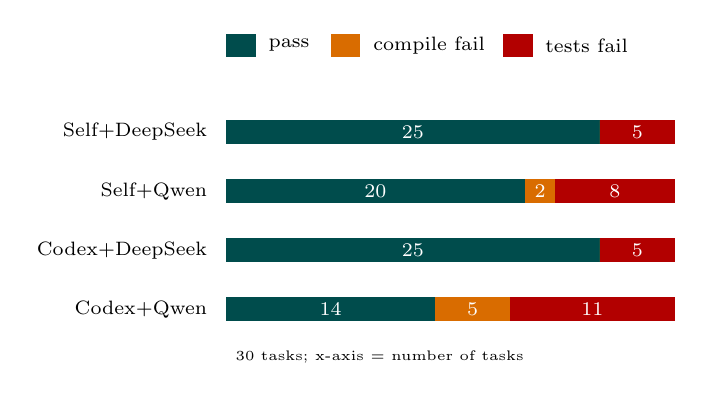
\begin{tikzpicture}[x=0.19cm,y=1cm]
        % legend
        \fill[teal!60!black] (0,0.55) rectangle (2,0.85);
        \node[anchor=west,font=\scriptsize] at (2.2,0.70) {pass};
        \fill[orange!85!black] (7,0.55) rectangle (9,0.85);
        \node[anchor=west,font=\scriptsize] at (9.2,0.70) {compile fail};
        \fill[red!70!black] (18.5,0.55) rectangle (20.5,0.85);
        \node[anchor=west,font=\scriptsize] at (20.7,0.70) {tests fail};

        \foreach \i/\name/\a/\b/\c in {%
            0/Self+DeepSeek/25/0/5,
            1/Self+Qwen/20/2/8,
            2/Codex+DeepSeek/25/0/5,
            3/Codex+Qwen/14/5/11}{%
          \node[anchor=east,font=\scriptsize] at (-0.6,{-\i*0.75-0.4}) {\name};
          \fill[teal!60!black]   (0,{-\i*0.75-0.55}) rectangle (\a,{-\i*0.75-0.25});
          \fill[orange!85!black] (\a,{-\i*0.75-0.55}) rectangle ({\a+\b},{-\i*0.75-0.25});
          \fill[red!70!black]    ({\a+\b},{-\i*0.75-0.55})
                                 rectangle ({\a+\b+\c},{-\i*0.75-0.25});
          \node[font=\scriptsize,text=white] at ({\a/2},{-\i*0.75-0.4}) {\a};
          \ifnum\b>0
            \node[font=\scriptsize,text=white] at ({\a+0.5*\b},{-\i*0.75-0.4}) {\b};
          \fi
          \node[font=\scriptsize,text=white] at ({\a+\b+0.5*\c},{-\i*0.75-0.4}) {\c};
        }
        \node[anchor=north west,font=\tiny] at (0,-3.05) {30 tasks; x-axis = number of tasks};
      \end{tikzpicture}}
    \end{column}
    \begin{column}{0.49\textwidth}
      \begin{itemize}
        \item On DeepSeek both frameworks have \textbf{zero} compile failures:
              the compile gate is no longer the bottleneck, all losses are
              behavioural
        \item Self-built + Qwen leaves only 2 tasks uncompilable, feedback pushes
              the other 28 into testing
        \item Codex + Qwen has \textbf{5 tasks still failing to compile}:
              30\% first round, so the 5-round budget burns on syntax
        \item Among compilable tasks the behavioural pass rates are
              83.3\% / 83.3\% / 71.4\% / 56.0\%: on Qwen the gap narrows
              \textbf{from 20 points to 15}, the rest comes from tasks that
              never compiled
      \end{itemize}
    \end{column}
  \end{columns}
\end{frame}

\begin{frame}
  \frametitle{Why 2: Where the Qwen Gap Comes From}

  \begin{columns}[T]
    \begin{column}{0.52\textwidth}
      \centering
      \small
      \setlength{\tabcolsep}{3.5pt}
      \begin{tabular}{@{}lcc@{}}
        \hline
        Metric (Qwen) & Self-built & Codex \\
        \hline
        Reach compiler, 1st round & \textbf{30/30} & \textbf{21/30} \\
        \quad blocked, interface check & 0 & 7 \\
        \quad blocked, block parsing   & 0 & 2 \\
        Compile errors per round       & \textbf{1.17} & \textbf{2.66} \\
        1st-round errors (med./mean)   & 0 / 1.2 & 2 / 3.7 \\
        Compiles on 1st round          & 23/30 & 9/30 \\
        Avg.\ rounds, tasks both pass  & \textbf{1.38} & \textbf{2.00} \\
        \hline
      \end{tabular}

      \vspace{2mm}
      \raggedright\small
      The failing sets largely overlap --- Codex needs \textbf{more rounds to
      converge at the same capability} (limit: 5).
    \end{column}
    \begin{column}{0.48\textwidth}
      \footnotesize
      \begin{itemize}
        \item \textbf{Output structure does not hold}: Codex emits
              \texttt{REAL}/\texttt{BOOL} as DUT names, array aliases as
              \texttt, or no POU block at all ---
              9 submissions never reached the compiler
        \item \textbf{Errors look C-like}: \texttt{C189} 74, \texttt{C9} 68
              samples read \texttt{expected ',' instead of ')'} or
              \texttt{instead of '!'} --- ST written as C/JS
              (\texttt{!}, \texttt{if(...)}, \texttt{//})
        \item \textbf{Prompt layer dilution}: Codex runs as a general agent, so
              the model must satisfy both ``I am a coding agent'' and ``emit one
              FB in a strict block format''; Qwen follows instructions weakly
              and slides to generic style --- why DeepSeek ties and Qwen
              diverges
        \item \textbf{Context layer}: median input 11,314 vs 1,573 tokens
              (7.2$\times$), squeezing the output budget (3,354 vs 6,101)
      \end{itemize}
    \end{column}
  \end{columns}

\end{frame}

% ============================================================
\section{Conclusion}

\begin{frame}
  \frametitle{Conclusion}

  \begin{enumerate}
    \item A 30-task dataset with per-task LTL specs, test cases (each step with a
          stated purpose) and reference implementations; all 30/30 compile and
          pass simulation
    \item The harness matches Codex on DeepSeek (83.3\% tests pass) at roughly
          1/7 of the input tokens and 1/2 of the wall time; on Qwen it is still
          better (66.7\% vs 46.7\%)
    \item The gap lies mainly in \textbf{the share that reaches the compiler}
          (30/30 vs 21/30), error density per round (1.17 vs 2.66) and context
          cost --- not in ``the model thinking too little''
  \end{enumerate}

  \vspace{0.2mm}
  \begin{block}{Limitations}
    \small
    \begin{itemize}
      \item Specs are not hooked to PLCVerif (optional item, not done); one
            sample per task, and the Qwen difference has Fisher exact
            $p=0.19$, not significant at the 0.05 level
      \item 12 scan steps carry no assertion and 34 BOOL inputs are never set
            TRUE, so pass rates hold ``under the current test cases''
      \item Next: PLCVerif integration, stronger case coverage, other platforms
    \end{itemize}
  \end{block}

  \vspace{0.6em}
  \begin{center}\footnotesize
    \begin{minipage}{0.92\textwidth}\centering
      Turning ``does it compile and does it run correctly'' into structured
      feedback lifts weak models; but no framework is better for every model.
    \end{minipage}
  \end{center}
\end{frame}

\end{document}
